\documentclass[tikz, border=10pt]{standalone}
\usepackage[utf8]{inputenc}
\usepackage{tikz}
\usetikzlibrary{shapes, arrows.meta, positioning, calc}
\usepackage{cjhebrew} % Attempt to use cjhebrew for simple Hebrew if installed, but might cause issues.
% Actually, let's just use English.

\begin{document}
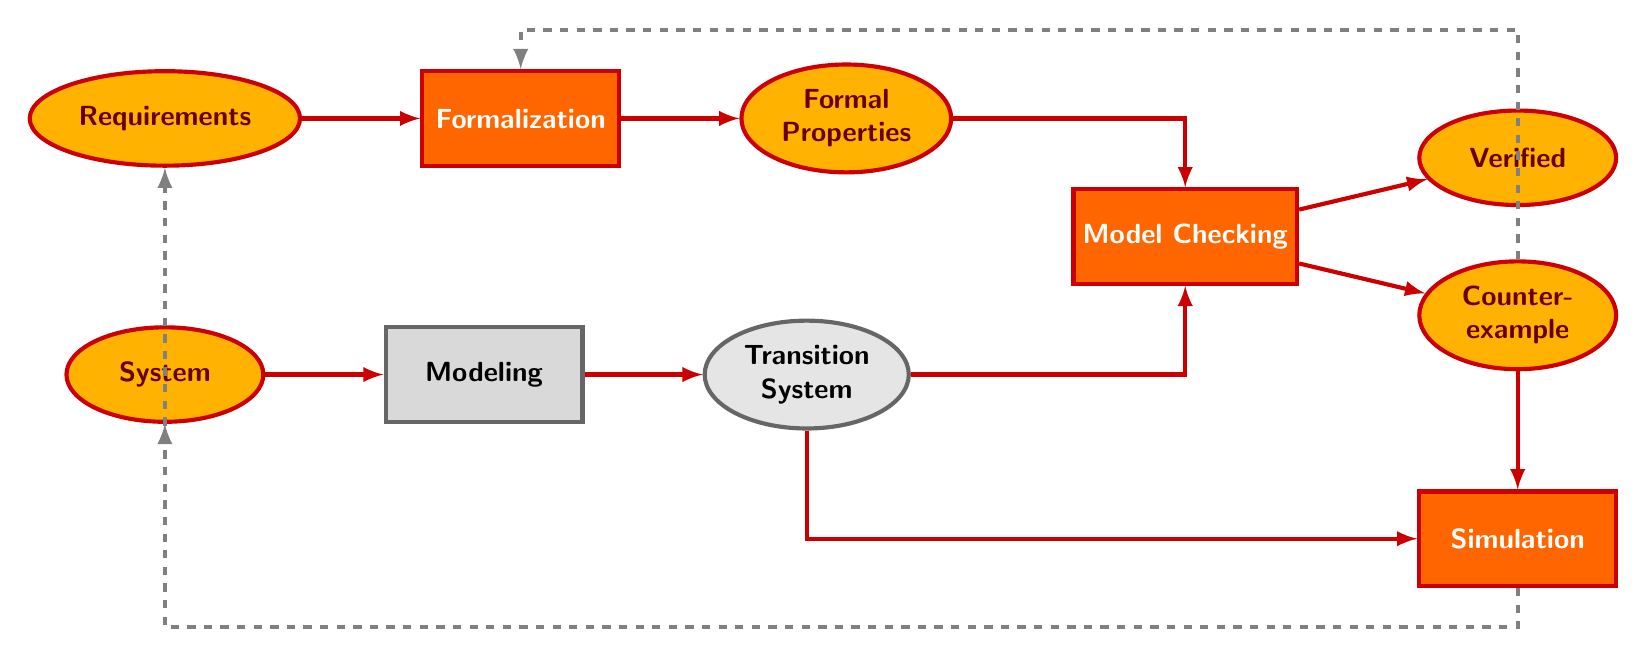
\begin{tikzpicture}[
    node distance=1.5cm and 1.5cm,
    font=\sffamily\bfseries,
    % Define styles
    block/.style={
        rectangle, 
        draw=red!80!black, 
        fill=orange!80!red, 
        text=white, 
        minimum width=2.5cm, 
        minimum height=1.2cm, 
        align=center,
        line width=1.5pt
    },
    oval/.style={
        ellipse, 
        draw=red!80!black, 
        fill=orange!60!yellow, 
        text=red!40!black, 
        minimum width=2.5cm, 
        minimum height=1.2cm, 
        align=center,
        line width=1.5pt
    },
    grayblock/.style={
        rectangle, 
        draw=gray!80!black, 
        fill=gray!30, 
        text=black, 
        minimum width=2.5cm, 
        minimum height=1.2cm, 
        align=center,
        line width=1.5pt
    },
    grayoval/.style={
        ellipse, 
        draw=gray!80!black, 
        fill=gray!20, 
        text=black, 
        minimum width=2.5cm, 
        minimum height=1.2cm, 
        align=center,
        line width=1.5pt
    },
    line/.style={
        draw, 
        -latex, 
        line width=1.5pt, 
        red!80!black
    },
    dashedline/.style={
        draw, 
        -latex, 
        dashed,
        line width=1.5pt, 
        gray
    }
]

% Place nodes
% Top row: Requirements -> Formalization -> Properties
\node[oval] (req) {Requirements};
\node[block, right=of req] (form) {Formalization};
\node[oval, right=of form] (props) {Formal\\Properties};

% Bottom row: System -> Modeling -> Transition System
\node[oval, below=2cm of req] (sys) {System};
\node[grayblock, right=of sys] (mod) {Modeling};
\node[grayoval, right=of mod] (ts) {Transition\\System};

% Middle: Model Checking
\node[block, right=1.5cm of props, yshift=-1.5cm] (mc) {Model Checking};

% Output
\node[oval, right=1.5cm of mc, yshift=1cm] (ver) {Verified};
\node[oval, right=1.5cm of mc, yshift=-1cm] (ce) {Counter-\\example};

% Simulation
\node[block, below=1.5cm of ce] (sim) {Simulation};


% Draw edges
% Top flow
\path[line] (req) -- (form);
\path[line] (form) -- (props);
\path[line] (props) -| (mc);

% Bottom flow
\path[line] (sys) -- (mod);
\path[line] (mod) -- (ts);
\path[line] (ts) -| (mc);

% Outputs
\path[line] (mc) -- (ver);
\path[line] (mc) -- (ce);

% Simulation flow
\path[line] (ts.south) |- (sim.west);
\path[line] (ce) -- (sim);

% Feedback loops
\path[dashedline] (sim.south) -- ++(0,-0.5) -| ($(sys.south)+(0,-0.5)$) -- (sys.south);
\path[dashedline] (sim.south) -- ++(0,-0.5) -| ($(req.south)+(0,-0.5)$) -- (req.south);
\path[dashedline] (ce.north) |- ($(form.north)+(0,0.5)$) -- (form.north);

\end{tikzpicture}
\end{document}
